\documentclass{beamer}
\usepackage[utf8]{inputenc}
\usepackage{tikz}
\usepackage{verbatim}
\usetheme{Darmstadt}
\title{Introduction to CouchDB}
\author{Ondřej Kupka}

\AtBeginSection[]
{
  \begin{frame}<beamer>
    \frametitle{Section Layout}
    \tableofcontents[currentsection]
  \end{frame}
}

\begin{document}

\begin{frame}
\titlepage
\end{frame}

\section{The Big Picture}
\subsection{Current Situation}
\begin{frame}{Current Situation on the Databases Market}
  \begin{itemize}
    \item RDBMS are de facto an industrial standard
    \begin{itemize}
      \item Solid theoretical background
      \item Implementations proven by time
      \item Commercial support provided by large companies
      \item Widespread
    \end{itemize}
    \item RDBMS do have something to offer
    \begin{itemize}
      \item Suitable for any data model that can be captured in relations
      \item Ad-hoc queries (run time flexibility)
      \item Consistency (transactions)
    \end{itemize}
  \end{itemize}
\end{frame}

\begin{frame}{New Challenges}
  With the advent of web-scale applications, we are facing many new~challenges.
  Huge amount of loosely structured data needs to~be processed.
  What we seek is:
  \begin{itemize}
    \item Good scalability while retaining consistency
    \item High performance
    \item High availability and robustness
  \end{itemize}
  We are, however, not living in a dreamworld \ldots
\end{frame}

\subsection{The Big Picture}
\begin{frame}{CAP (Brewer's) Theorem}
  No distributed computer system can simultaneously provide\\all of
  the following guarantees:
  \begin{itemize}
    \item Consistency
    \item Availability
    \item Partition tolerance
  \end{itemize}
  \begin{center}
    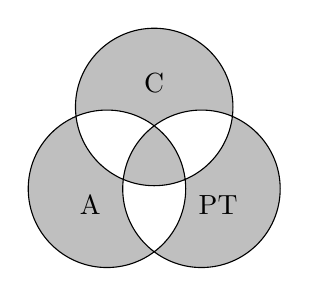
\begin{tikzpicture}
      \filldraw[fill=lightgray,even odd rule]
        (60:1.2) circle (1) ++(90:0.3) node{C}
        (0:0) circle (1) ++(225:0.3) node{A}
        (0:1.2) circle (1) ++(315:0.3) node{PT};
    \end{tikzpicture}
  \end{center}
  \fontsize{6}{8}\selectfont
  Began as a conjecture by Eric Brewer in 2000 and was proven by Seth Gilbert
  and Nancy Lynch of MIT in 2002.\\
\end{frame}

\begin{frame}{Consistency Model Revised}
  \begin{description}
    \item[ACID] (pesimistic - Consistency + Availability) \hfill
    \begin{enumerate}
      \item Atomicity
      \item Consistency
      \item Isolation
      \item Durability
    \end{enumerate}
    \item[BASE] (optimistic - Availability + Partition tolerance) \hfill
    \begin{enumerate}
      \item Basically Available
      \item Soft state
      \item Eventual consistency
    \end{enumerate}
  \end{description} 
\end{frame}

\subsection{The NoSQL Movement}
\begin{frame}{History and Core Principles}
  \begin{itemize}
    \item In 1998 Carlo Strozzi used the term to name light-weight DBs with no SQL,
          and also no relations. He then suggested to call them 'NoREL'.
    \item Reintroduced by Eric Evans of Rackspace in 2009 to name\\a growing
          number of non-relational distributed DBs\\not attemping to provide ACID.
    \item Today it is usually translated as 'Not only SQL'.
    \item In 2011, work began on UnQL, a query language for NoSQL databases.
          Does not cover the data definition.
  \end{itemize}
\end{frame}

\begin{frame}{Characteristics}
  Among the ideas characterizing NoSQL databases are:
  \begin{itemize}
    \item High optimisation for just the basic (CRUD) operations
    \item Providing little functionality beyond record storage
    \item Trading run time flexibility for gains in performance and scalability
          for certain data models (specialization)
    \item No SQL as the query language
    \item No ACID guarantees (BASE)
    \item Distributed and fault-tolerant
  \end{itemize}
  So basically we get systems that are hard to bring down and are able to handle
  enormous amount of data, but they are sacrificing functionality for that.
  If you, however, pick up the right system for you, it can do magic.
\end{frame}

\begin{frame}{Taxonomy of NoSQL Databases}
  \begin{itemize}
    \item Key-value stores
    \item \alert<2>{Document stores}
    \item Column families
    \item Graph databases
    \item Tuple/RDF stores
    \item XML databases
    \item Object stores
    \item \ldots
  \end{itemize}
\end{frame}

\begin{frame}[fragile]{Document Stores}
  You can imagine a document store as a key-value store,\\but the database begins
  to understand the structure of values (called 'documents') stored in there,
  which implies:
  \begin{itemize}
    \item Need for particular encoding of the data (XML, JSON, \ldots),
          but still no structure (no hard-coded schemas)
    \item It is possible to query the data (and do computations - MapReduce)
    \item It works in a CRUD way, a document is the basic unit.
          Operations on documents are usually the only atomic thing.
  \end{itemize}
  \fontsize{8}{10}\selectfont
  \begin{verbatim}
  { "firstName": "John", "lastName": "Smith" }
  \end{verbatim}
  Examples: MongoDB, \alert<2>{CouchDB}, RavenDB (transactions!)
\end{frame}

\section{CouchDB}
\subsection{Introduction}
\begin{frame}[fragile]{Before We Start}
  \framesubtitle{Installing and Starting CouchDB}
  Let us set up CouchDB so that we can try what we have learned immediately!
  Change defaults for production! There is a webmin called Futon
  bundled with CouchDB that you can use...
  \fontsize{6}{8}\selectfont
  \begin{verbatim}
  $ brew install couchdb # or apt-get install or whatever...
  $ couchdb
  Apache CouchDB 1.2.0 (LogLevel=info) is starting.
  Apache CouchDB has started. Time to relax.
  [info] [<0.31.0>] Apache CouchDB has started on http://127.0.0.1:5984/
  ...

  $ open http://127.0.0.1:5984/_utils # for Futon
  \end{verbatim}
\end{frame}

\begin{frame}{Overview and Core Features}
  \begin{itemize}
    \item Initial release in 2005, Apache project in 2008 (OSS)
    \item \textit{A database that completely embraces the web}
    \begin{itemize}
      \item Store JSON documents
      \item Access them via HTTP
      \item Query, combine and transform data with JavaScript
      \item Even serve applications directly out of CouchDB
    \end{itemize}
    \item ACID semantics (Multi-Version Concurrency Control)
    \item Eventual consistency
    \item Built for being offline (Partition tolerance)
    \item Distributed architecture with replication
    \item MapReduce views, and indexes
    \item REST API
  \end{itemize}
\end{frame}

\subsection{Document Storage}
\begin{frame}[fragile]{Basics}
  \begin{itemize}
    \item Server stores named databases, which contain\\JSON documents (mostly)
    \item Documents are primary units of data; they have any number of fields
          and attachments, and database metadata like id\\and revision
    \item Update model is optimistic and lockless
    \begin{itemize}
      \item load - modify - save not atomic, MVCC used to signal conflicts
    \end{itemize}
  \end{itemize}
  \fontsize{6}{8}\selectfont
  \begin{verbatim}
  {"_id":"89027e7860926e4815267048520017df","_rev":"1-bfb0d347cff4cb38161d90ea749fe2a0",
   "firstname":"Ondrej","surname":"Kupka"}
  \end{verbatim}
\end{frame}

\begin{frame}[fragile]{Demo 1 - Database and Document Creation}
  \fontsize{6}{8}\selectfont
  \begin{verbatim}
  $ curl -X PUT http://127.0.0.1:5984/testdb
  {"ok":true}
  $ curl -X GET http://127.0.0.1:5984/_uuids
  {"uuids":["89027e7860926e4815267048520017ec"]}
  $ curl -X PUT http://127.0.0.1:5984/testdb/89027e7860926e4815267048520017ec \
  > -d '{"firstname":"Ondrej","surname":"Kupka"}'
  {"ok":true,"id":"89027e7860926e4815267048520017ec","rev":"1-bfb0d347cff4cb38161d90ea749fe2a0"}
  \end{verbatim}
\end{frame}

\begin{frame}[fragile]{Demo 2 - Conflict Occurence and Resolution}
  \fontsize{6}{8}\selectfont
  \begin{verbatim}
  ME$ curl -X GET http://127.0.0.1:5984/testdb/89027e7860926e4815267048520017ec
  {"_id":"89027e7860926e4815267048520017ec","_rev":"1-bfb0d347cff4cb38161d90ea749fe2a0",
   "firstname":"Ondrej","surname":"Kupka"}

  HIM$ curl -X GET http://127.0.0.1:5984/testdb/89027e7860926e4815267048520017ec
  {"_id":"89027e7860926e4815267048520017ec","_rev":"1-bfb0d347cff4cb38161d90ea749fe2a0",
   "firstname":"Ondrej","surname":"Kupka"}

  HIM$ curl -X PUT http://127.0.0.1:5984/testdb/89027e7860926e4815267048520017ec \
  >  -d '{"_rev":"1-bfb0d347cff4cb38161d90ea749fe2a0","firstname":"Ondrej","surname":"Krupka"}'
  {"ok":true,"id":"89027e7860926e4815267048520017ec","rev":"2-e1db85ed9d716a6555736282d7bee514"}

  ME$ curl -X PUT http://127.0.0.1:5984/testdb/89027e7860926e4815267048520017ec \
  >  -d '{"_rev":"1-bfb0d347cff4cb38161d90ea749fe2a0","firstname":"Ondrej","surname":"Krupicka"}'
  {"error":"conflict","reason":"Document update conflict."}

  ME$ curl -X GET http://127.0.0.1:5984/testdb/89027e7860926e4815267048520017ec
  {"_id":"89027e7860926e4815267048520017ec","_rev":"2-e1db85ed9d716a6555736282d7bee514",
   "firstname":"Ondrej","surname":"Krupka"}

  ME$ curl -X PUT http://127.0.0.1:5984/testdb/89027e7860926e4815267048520017ec \
  > -d '{"_rev":"2-e1db85ed9d716a6555736282d7bee514","firstname":"Ondrej","surname":"Krupicka"}'
  {"ok":true,"id":"89027e7860926e4815267048520017ec","rev":"3-3182f9d7d36974848e9bcbb0f71dcfcc"}
  \end{verbatim}
\end{frame}

\begin{frame}{ACID Properties and Implementation Details}
  \begin{itemize}
    \item Commited data are never overwritten, appending only,\\always consistent
    \begin{enumerate}
      \item All data and updates flushed to the disk synchronously
      \item Updated DB header written in two consecutive, identical chunks
            to the beginning of the file, then flushed.
    \end{enumerate}
    \item Updates serialized except binary blobs
    \item B-tree indexes of documents (DocID, SeqID),\\B-trees everywhere
    \item Clients are never locked out - revision = consistent snapshot
    \item Compaction
    \item Written in Erlang/OTP - concurrent (actors), robust, share-nothing
  \end{itemize}
\end{frame}

\subsection{Querying and Manipulating Stored Data}
\begin{frame}{Design Documents}
\end{frame}

\begin{frame}{Views}
\end{frame}

\begin{frame}{List Functions}
\end{frame}

\begin{frame}{Show Functions}
\end{frame}

\subsection{Security and Validation}
\begin{frame}
\end{frame}

\begin{frame}{Validation Function}
\end{frame}

\subsection{Distributed Updates and Replication}
\begin{frame}
\end{frame}

\subsection{Applications}
\begin{frame}
\end{frame}

\subsection{When not to use CouchDB}
\begin{frame}
\end{frame}

\subsection{Developing with CouchDB}
\begin{frame}{Couchapps, Kanso and stuff}
\end{frame}

\subsection{Future Plans}
\begin{frame}
\end{frame}

\subsection{Resources}
\begin{frame}{Resources}
\end{frame}

\end{document}
